\section{Datasets}
\label{sec:datasets}
For testing the bootstrapping technique and curriculum learning as well as measuring the performance of the aerial patch framework, two datasets have been used. Both datasets involve learning structured output predictions from images, specifically the task of extracting roads from aerial images \todo{Weird sentence, do datasets involve or learning from these involve}. The first dataset, Massachusetts Roads Dataset, is provided by \cite{MnihThesis} and have been used in other works. The second dataset, Norwegian Roads Dataset, have been created from publicly available source specifically for this thesis. Differences, similarities and challenges of employing these datasets will be further discussed below.\\

\subsection{Massachusetts Roads Dataset}
The Massachusetts Roads Dataset contains aerial images depicting urban, suburban and rural areas in the state of Massachusetts, USA. In all the dataset consists of 1171 aerial images, where each image is $1500\times 1500$ pixels in size. The main bulk, or 1108 of these images have been randomly assigned to the training set. The remaining 49 and 14 images can be found in the test and validation set. The dataset covers an area of 2600 square kilometers in total, which gives a ground sampling distance of 1.0 meter per pixel.\\

Each aerial image have an accompanying identically sized binary label image which indicate whether a pixel in the aerial image contains a road or not \todo{rewrite this sentence}. Road centerline vectors retrieved from the OpenStreetMap project were used to generate the labels images \citep{MnihThesis}. The vectors were rasterized as white lines with a line thickness of 7 pixels. An example from this dataset can be seen in Figure \ref{fig:mass_roads_example}.  \\

\begin{figure}
\begin{subfigure}{0.48\textwidth}
\includegraphics[width=\linewidth]{figs/datasets/Mass_roads_data_example.png}
\caption{Aerial image} \label{fig:mass_roads_example_data}
\end{subfigure}
\hspace*{\fill} % separation between the subfigures
\begin{subfigure}{0.48\textwidth}
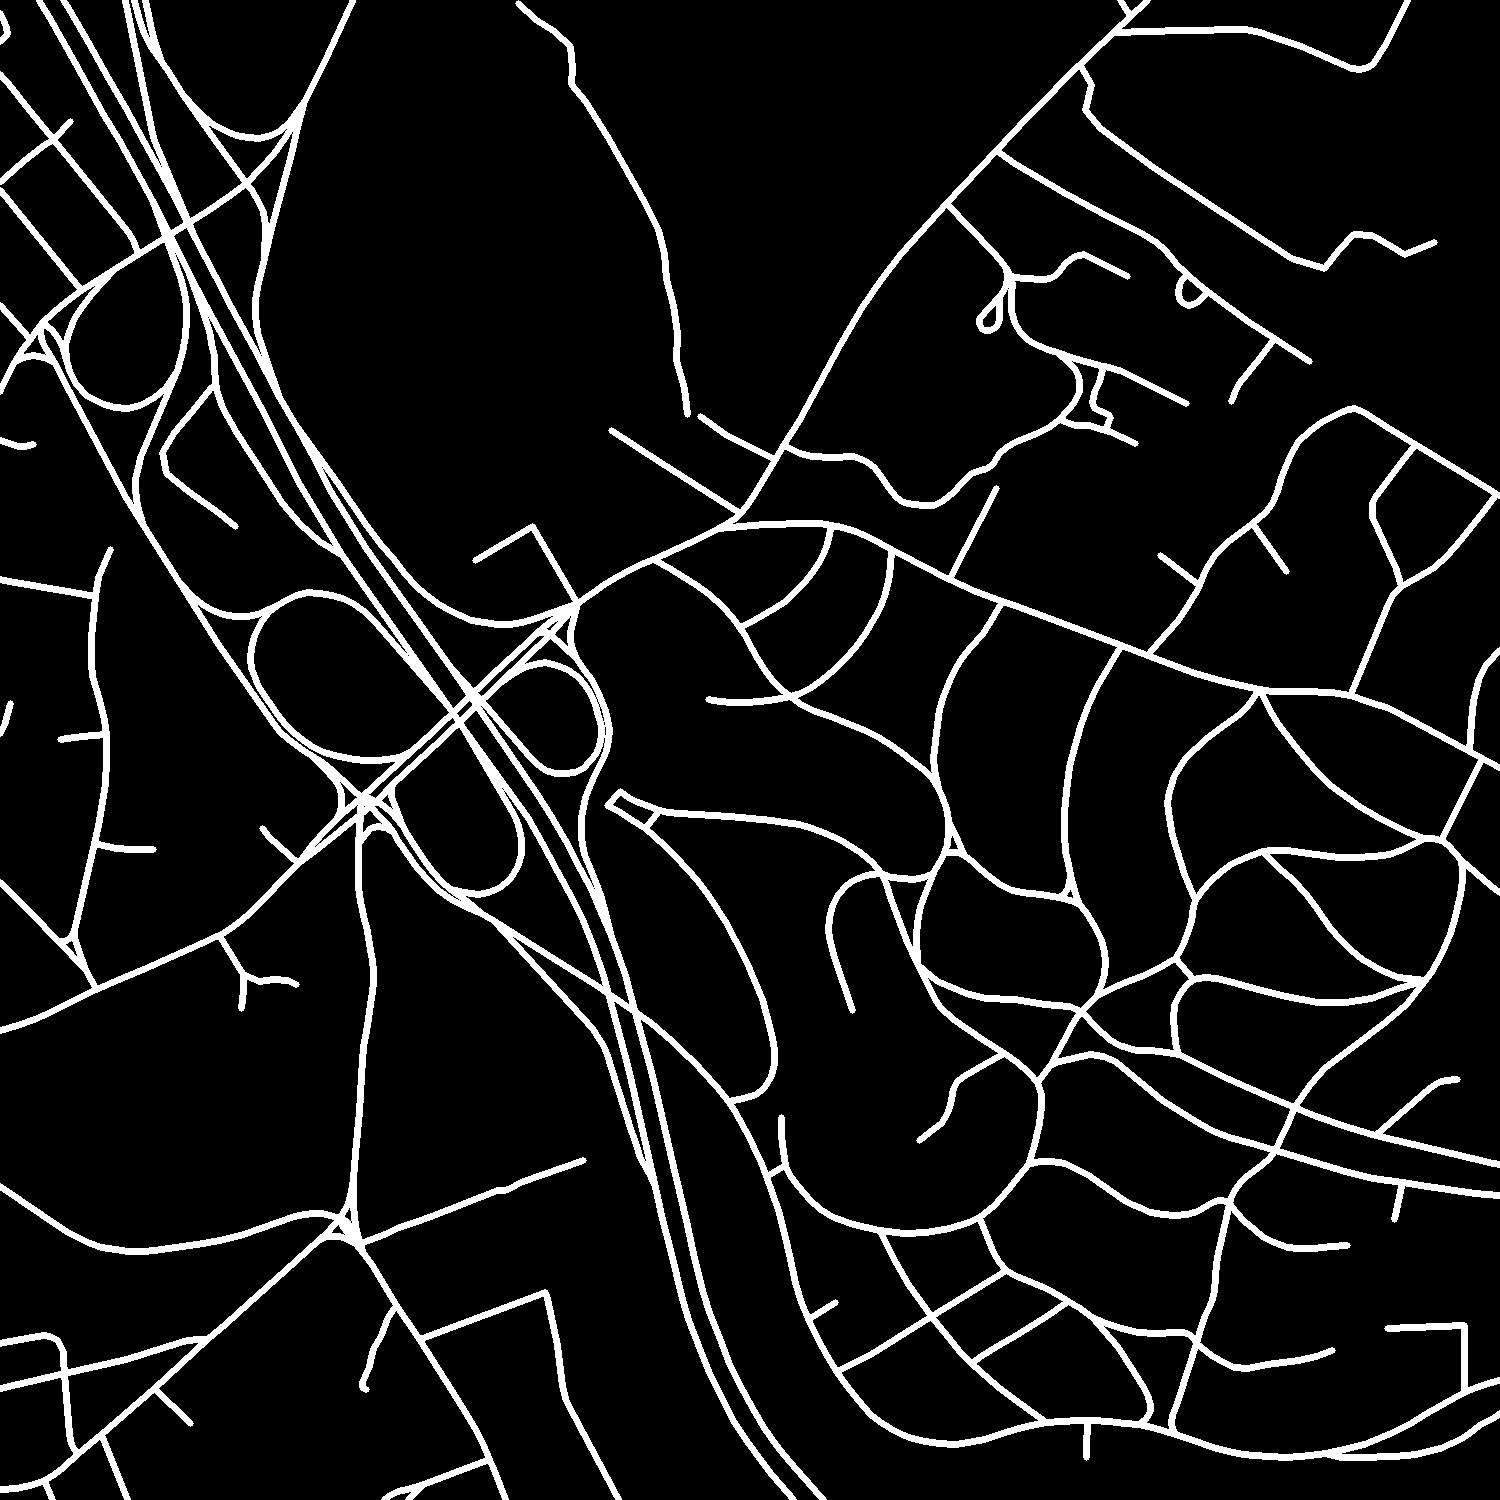
\includegraphics[width=\linewidth]{figs/datasets/Mass_roads_label_example.png}
\caption{Label image} \label{fig:mass_roads_example_label}
\end{subfigure}
\hspace*{\fill} % separation between the subfigures
\caption{Example taken from test set in Massachusetts Roads Dataset} \label{fig:mass_roads_example}
\end{figure}


\todo[inline]{Challenges with this particular dataset. And why it has been chosen}



%\subsection{Massachusetts Roads Dataset}
\todo[inline]{Include buildings dataset or not?}
\subsection{Norwegian Roads Dataset}

This dataset presents some challenges in terms of label resolution. Road labels registration errors. Fewer omission errors.
Road labels not generated with uniform breadth. Road labels more accurate in terms of road breadth. Images taken mainly from urban and suburban areas throughout norway. In terms of typograhy (Right word?). Cultivated land, mountains, ice, forest areas. Images also range in quality. Different color hues. Vegvesenet --
Ground sampling distance of 0.66. 
The dataset covers an area of approximately 
1200 km2.\\

In addition to the Massachusetts Roads Dataset \citep{MnihThesis}, the proposed algorithm will be tested on a new dataset. This dataset was constructed from aerial images retrieved from Kartverket, which depicts both rural and urban areas in Norway. The labels for this dataset have been generated from road center-line vectors found in the publicly available topographic vector database, N50, provided by Kartverket. \\

Currently, the dataset contains 221 RGB images that are 1536 pixels in width and height. The images have a high resolution with a \ac{GSD} of around 0.66 meters per pixel. There are 184 images in the training set, 21 images in the validation set, and 16 images in the test set. The road center-line vectors are generated as 4 pixel wide black lines in the label images. A cropped image from this dataset can be seen in Figure \ref{fig:aerialimage_norwegian}, with the label image superimposed on the aerial image. Observe that some roads are missing from the label image, as well as the ground truth not covering the roads properly. \\

\begin{figure}
\begin{subfigure}{0.32\textwidth}
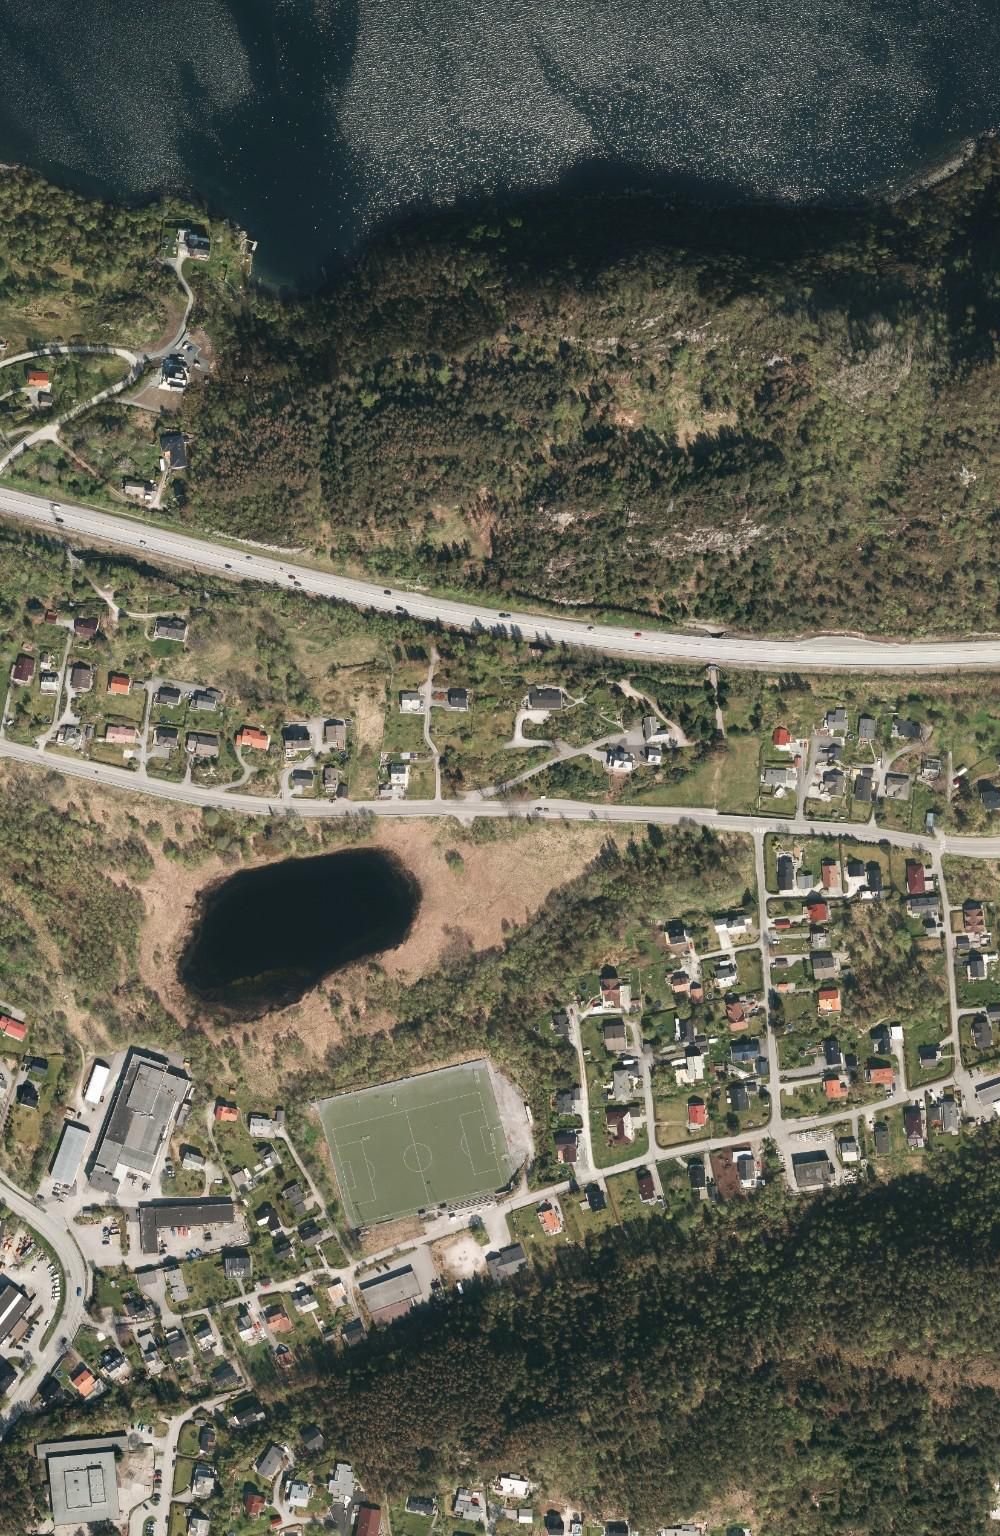
\includegraphics[width=\linewidth]{figs/datasets/Norwegian_roads_data_example.png}
\caption{Aerial image} \label{fig:norwegian_roads_example_data}
\end{subfigure}
\hspace*{\fill} % separation between the subfigures
\begin{subfigure}{0.32\textwidth}
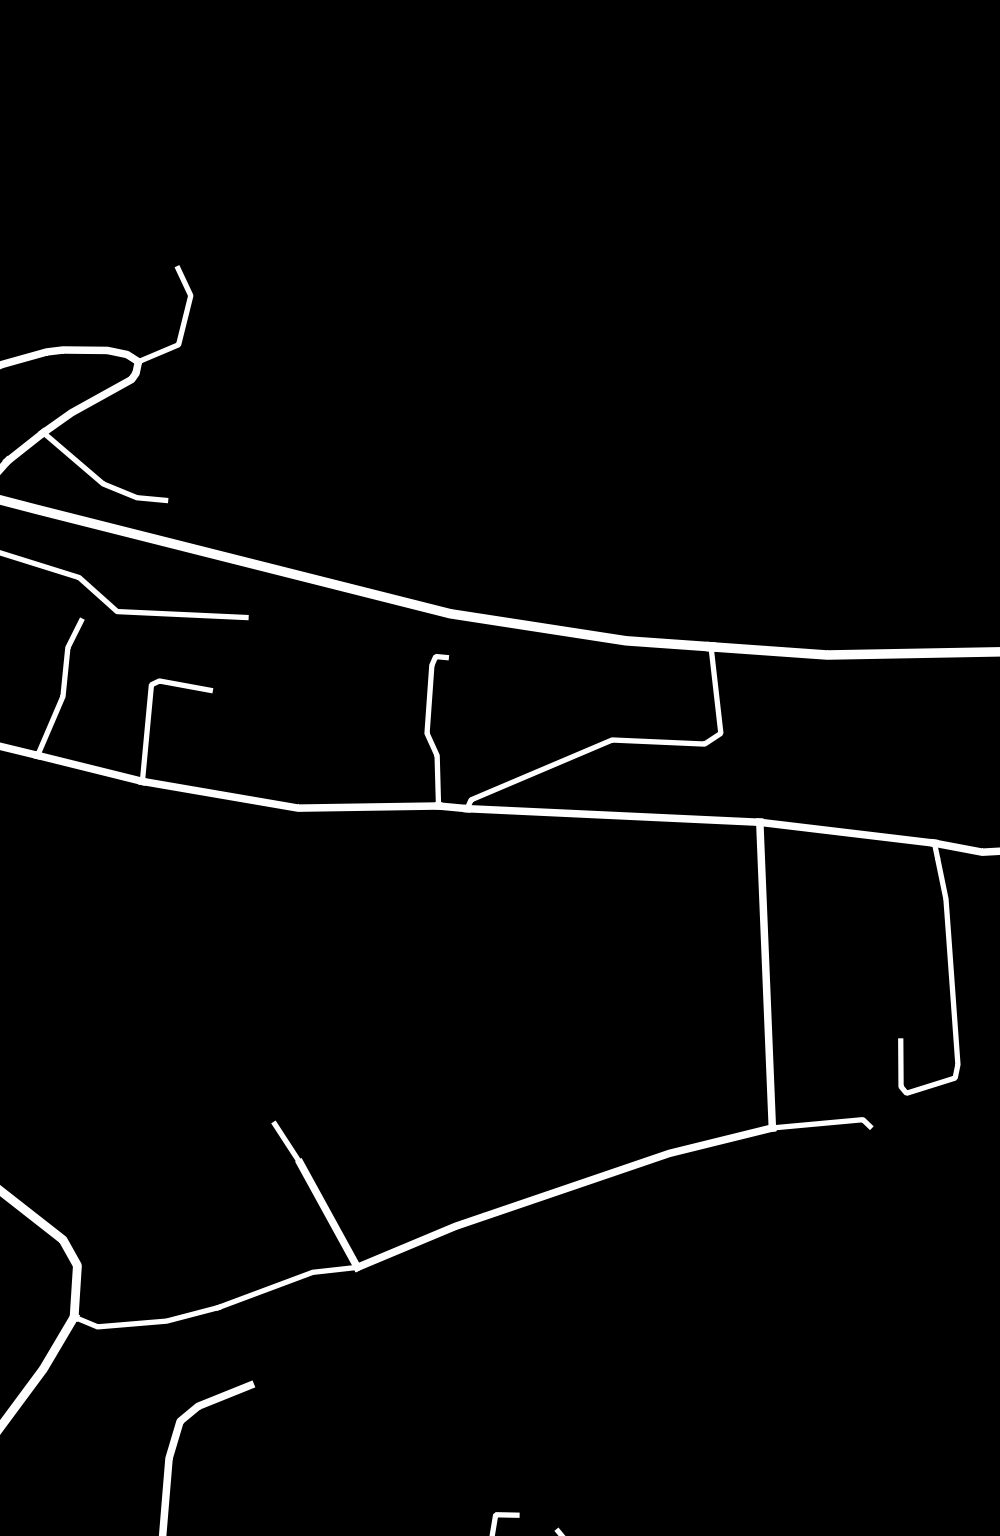
\includegraphics[width=\linewidth]{figs/datasets/Norwegian_roads_label_example.png}
\caption{Label image} \label{fig:norwegian_roads_example_label}
\end{subfigure}
\hspace*{\fill} % separation between the subfigures
\begin{subfigure}{0.32\textwidth}
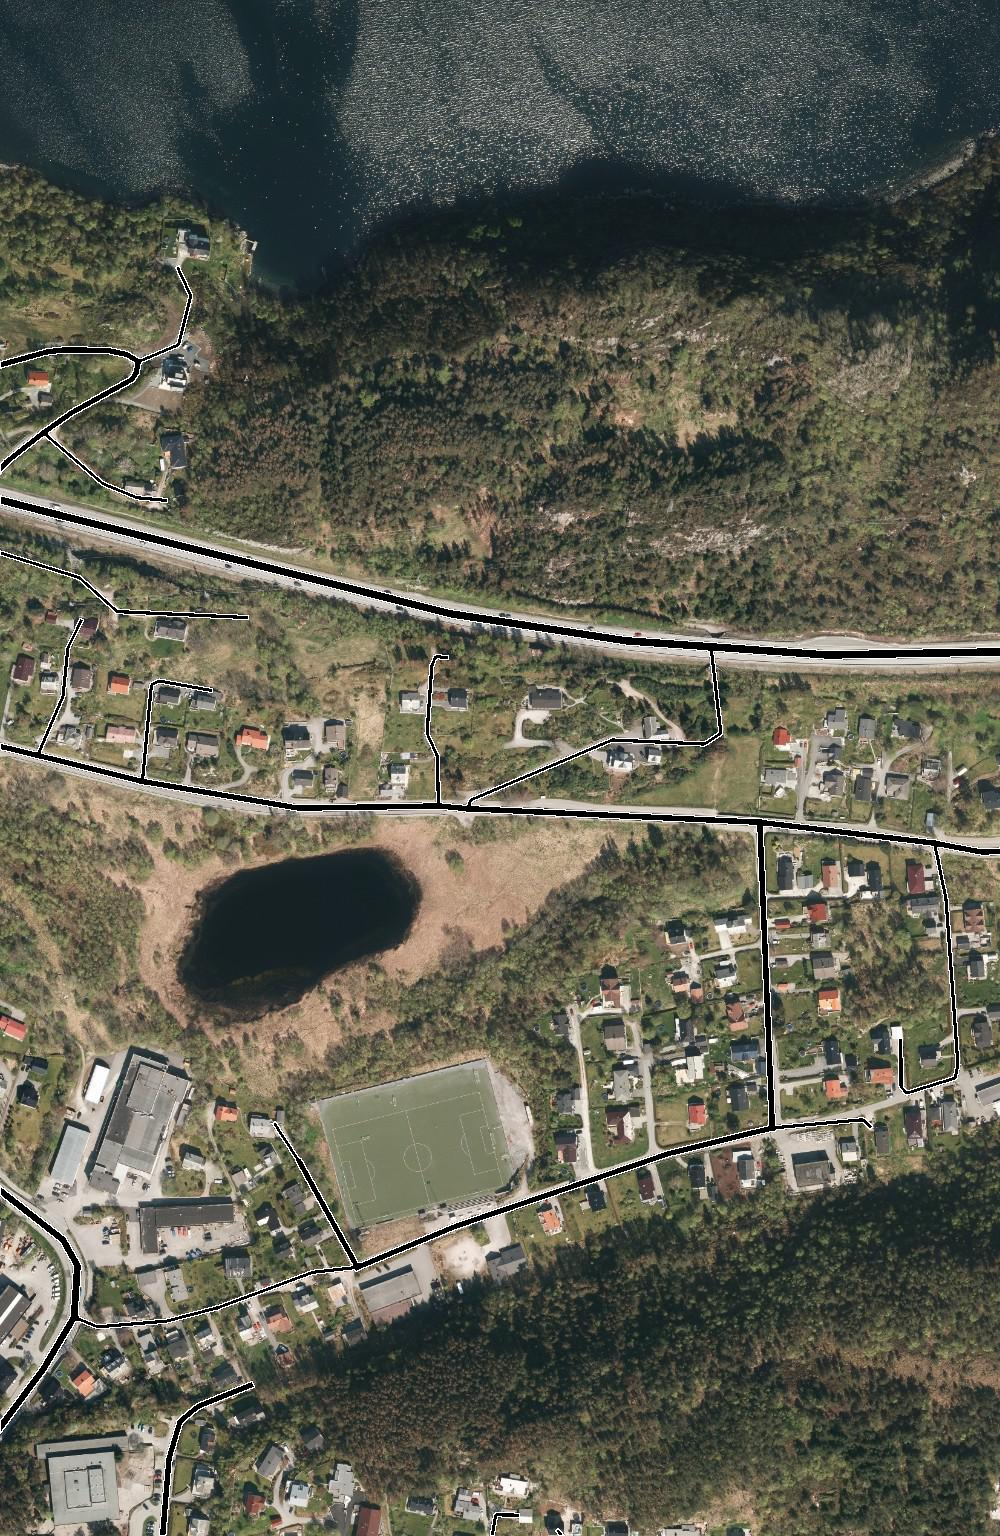
\includegraphics[width=\linewidth]{figs/datasets/Norwegian_roads_overlay_example.png}
\caption{Overlay} \label{fig:norwegian_roads_example_overlay}
\end{subfigure}
\hspace*{\fill} % separation between the subfigures
\caption{Example taken from test set in Norwegian Roads Dataset} \label{fig:norwegian_roads_example}
\end{figure}

\begin{figure}[t]
\begin{center}
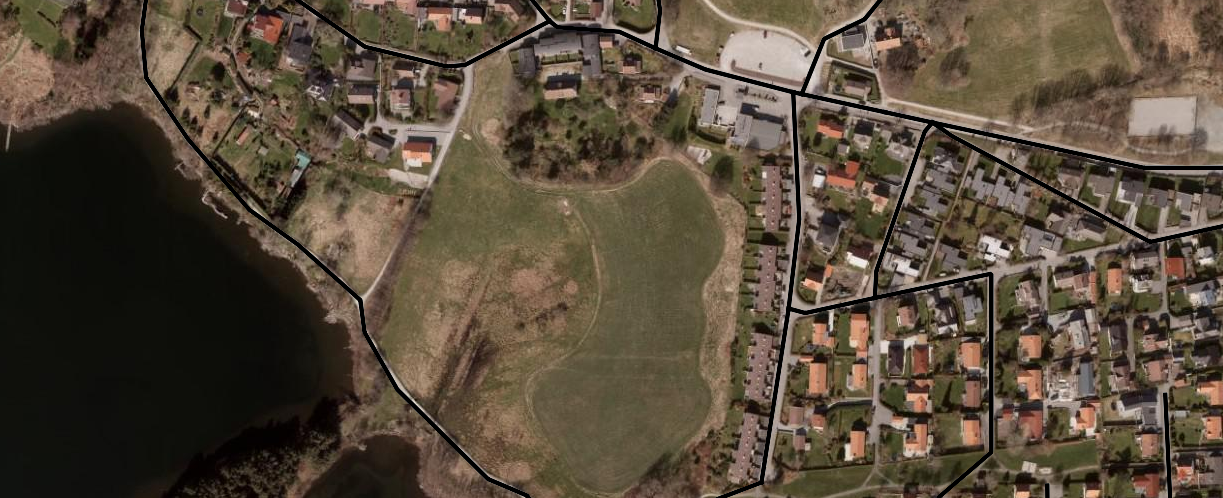
\includegraphics[width=1\columnwidth]{figs/norwegian_dataset.png}
\caption[Norwegian road dataset example]{Example aerial image with the label image as an overlay.}
\label{fig:aerialimage_norwegian}
\end{center}
\end{figure}

The Norwegian Roads Dataset has been constructed by using QGIS, an open source geographic information system application. The application enables viewing and editing of map data, but also provides a Python interface. A script to create label images was developed, which takes the map coordinates associated with each corner of an aerial image, and generates a raster image of road center-line vectors found inside that area. These raster images can be used as label data in supervised learning. \\

Oppskrift
teknisk fakta om datasettet. Hvor store, gi et eksempel, hvor mange og hvordan de er fordelt i test , trainnig og validation 
Geo-teknisk. Hvor stort område dekker datasettet, og hvor tykke er vei linjene
Utfordringer - omission etc etc.
random utvalg - gir 25\% med vei -etc etc